\ifdefined\COMPLETE
\else
\documentclass[12pt]{article}
\usepackage{tikz}
\usepackage{color}

\usetikzlibrary{shapes, calc, arrows, through, intersections, decorations.pathreplacing, patterns}

\begin{document}
\fi
\def\alph{$2$}
\def\a{$2$}
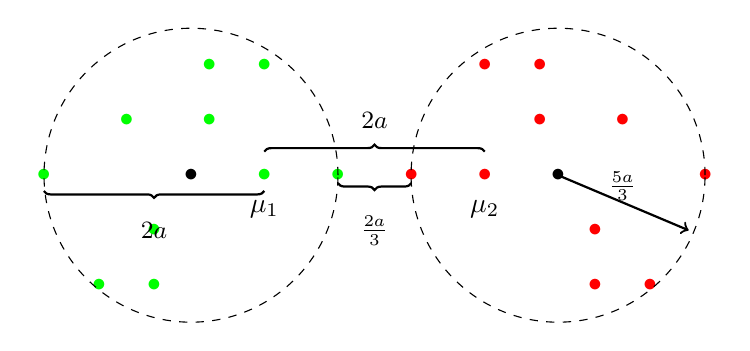
\begin{tikzpicture}[scale=7]
	\coordinate (x) at ($ (-0.02,{sqrt(0)}) $);
	\coordinate (y) at (2.1,0);

	\node[green] at (-0.45,0.1) {$\bullet$};
	\node[green] at (-0.4,-0.10) {$\bullet$};
	\node[green] at (-0.3,0.1) {$\bullet$};
	\node[green] at (-0.5,-0.2) {$\bullet$};
	\node[green] at (-0.4,-0.2) {$\bullet$};
	\node[green] at (-0.3,0.2) {$\bullet$};
	\node[green] at (-0.2,0.2) {$\bullet$};
	
	\node at (-0.333,0) {$\bullet$};
	\node[green,label=270:$\mu_1$] at (-0.2,0) {$\bullet$};
	\node[green] at (-0.06666,0) {$\bullet$};
	\node[green] at (-0.6,0) {$\bullet$};
	
	\node at (0.333,0) {$\bullet$};
	\node[red,label=270:$\mu_2$] at (0.2,0) {$\bullet$};
	\node[red] at (0.06666,0) {$\bullet$};
	\node[red] at (0.6,0) {$\bullet$};
	
	\node[red] at (0.45,0.1) {$\bullet$};
	\node[red] at (0.4,-0.10) {$\bullet$};
	\node[red] at (0.3,0.1) {$\bullet$};
	\node[red] at (0.5,-0.2) {$\bullet$};
	\node[red] at (0.4,-0.2) {$\bullet$};
	\node[red] at (0.3,0.2) {$\bullet$};
	\node[red] at (0.2,0.2) {$\bullet$};

	\node at (0.0,0.1) {\small{$2a$}};
	\node at (0.0,-0.1) {\small{$\frac{2a}{3}$}};
	\node at (-0.4,-0.1) {\small{$2a$}};
	\node at (0.45,-0.02) {\small{$\frac{5a}{3}$}};

	\draw[black, dashed] (-0.333,0.0) circle (0.266666);
	\draw[black, dashed] (0.333, 0.0) circle (0.266666);

	\draw[thick,->] (0.333, 0) -- (0.57, -0.1);
	\draw [thick, decoration={brace, mirror, raise=0.1cm}, decorate ] (-0.0666, 0) -- (0.06666, 0); 
	\draw [thick, decoration={brace, raise=0.3cm}, decorate ] (-0.2, 0) -- (0.2, 0); 
	\draw [thick, decoration={brace, raise=0.2cm}, decorate ] (-0.2, 0) -- (-0.6, 0); 
	
\end{tikzpicture}


\ifdefined\COMPLETE
\else
\end{document}
\fi
